% !TEX root = omar-thesis-proposal.tex
\section{Active Code Completion}\label{acc}
A language's syntax and semantics influences the behavior of a variety of tools beyond the compiler. For example, software developers today make heavy use of the code completion support found in modern source code editors  \cite{murphy_how_2006}. Editors for object-oriented languages provide code completion in the form of a floating menu containing  contextually-relevant variables, fields, methods, types and other code snippets. By navigating and selecting from this menu, developers are able to avoid many common spelling and logic errors, eliminate unnecessary keystrokes and explore unfamiliar APIs without incurring the mental overhead associated with switching to an external documentation tool.
% The way code completion menus brought documentation systems into the editor, active code completion interfaces bring external tools into the editor.

%Several refinements and additions to the code completion menu have previously been suggested in the literature. These have focused on leveraging additional sources of information, such as databases of usage history \cite{robbes_how_2008}\cite{HouPletcher2011}, inheritance information \cite{HouPletcher2011}, API-specific information \cite{HouPletcher2011}\cite{Lee+2008}, partial abbreviations \cite{Han+2009}, examples extracted from code repositories \cite{bruch_learning_2009}\cite{Brandt+2010} and crowdsourced information \cite{mooty_calcite:_2010}\cite{SnipMatch}, to increase the relevance and sophistication of the featured menu items. As with the standard form of code completion, many of these sources of data can also be utilized via external tools (e.g. Calcite \cite{mooty_calcite:_2010} uses information that could already be accessed using the Jadeite \cite{conf/vl/StylosFYM09} tool). Empirical evidence presented in these studies, however, suggests that directly integrating these kinds of tools into the editor is particularly effective. For example, users of the Calcite tool completed 40\% more tasks in a lab study (unfortunately, a Jadeite control group was not included.)

In all such systems, the code completion interface has remained primarily menu-based. When an item in the menu is selected, code is inserted immediately, without further input from the developer. These systems are difficult to extend: a fixed strategy determines the completions that are available, so library providers cannot directly specify new domain-specific or contextually-relevant logic or provide assistance beyond that which a menu can provide. 
In this paper we propose a technique called {\it active code completion} that eliminates these restrictions using active types. This  makes developing and integrating a broad array of highly-specialized code generation tools directly into the editor, via the familiar code completion command, significantly simpler.% This technique is motivated by the evidence discussed above and further evidence provided in this paper that developers prefer, and make more effective use of, tools that do not require leaving the immediate editing environment.

In this work, we discuss active code completion in the context of object construction in Java because type-aware editors for Java are better developed than those for other languages, because we wish to do empirical studies, and because Java already provides a way to associate metadata with classes. The techniques in this section apply equally well to type-aware editors for any language with a similar mechanism. 

For example, consider the following Java code fragment:

\begin{lstlisting}
  public Color getDefaultColor() {
      return _
\end{lstlisting}

\begin{figure*}\label{color}
\begin{center}
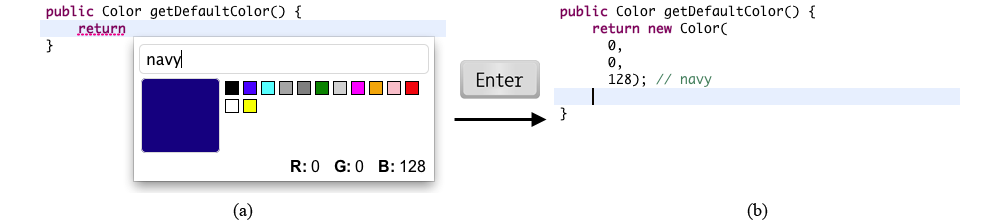
\includegraphics[width=40pc]{color_palette.png}\end{center}
\caption{(a) An example code completion palette associated with the \texttt{Color} class. (b) The source code generated by this palette.}
\label{colorpalette}
\end{figure*}

If the developer invokes the code completion command at the indicated cursor position (\li{_}), the editor  looks  for a {\it palette definition} associated with the {\it type} of the expression being entered, which in this case is  \verb|Color|. If an associated palette is found, a menu item briefly describing this palette is added to the standard code completion menu. When selected, the corresponding palette is shown, replacing the standard code completion menu. Figure \ref{colorpalette}(a) gives an example of a simple palette that may be associated with the \verb|Color| class\footnote{A video demonstrating this process is available at \url{http://www.cs.cmu.edu/~NatProg/graphite.html}.}. 

The developer can interact with such palettes to provide parameters and other information related to their intent, and receive immediate feedback about the effect these choices will have on the behavior of the object being constructed. When this interaction is complete, the palette generates appropriate source code for insertion at the cursor. Figure \ref{colorpalette}(b) shows the inserted code after the user presses \textsc{enter}.

We sought to address the following questions before designing and implementing our active code completion system:

\begin{itemize}
\item What {\it specific} use cases exist for this form of active code completion in a professional development setting? 
\item What {\it general} criteria are common to types that would and would not benefit from an associated palette?
\item What are some relevant usability and design criteria for palettes designed to address such use cases?
\item What capabilities must the underlying active code completion system provide to enable these use cases and user interface designs?
\end{itemize}

To help us answer these questions, we conducted a survey of 473 professional developers. Their responses, along with information gathered from informal interviews and code corpus analyses, revealed a number of non-trivial functional requirements for palette interfaces as well as the underlying active code completion architecture. Participants also suggested a large number of use cases, demonstrating the broad applicability of this technique. We organized these into several broad categories. Next, we developed Graphite, an Eclipse plug-in that implements the active code completion architecture for the Java programming language, allowing Java library developers to associate custom palettes with their own classes. We describe several design choices that we made to satisfy the requirements discovered in our preliminary investigations and examine necessary trade-offs. Finally, we conducted a pilot lab study with a more complex palette, implemented using Graphite, that assists developers as they write regular expressions. The study provides specific evidence in support of the broader claim that highly-specialized tools that are integrated directly with the editing environment are  useful. We conclude that active code completion systems like Graphite are useful because they make developing, deploying and discovering such tools fundamentally simpler.

The primary concerns relevant to this thesis are:
\begin{itemize}
\item The palette mechanism should not be tied to a specific editor implementation. We achieve this by using a URL-based scheme for referring to palettes, which are implemented as webpages, which can be embedded into any editor using standard techniques for embedding browsers into GUIs.
\item The palette mechanism should not be able to arbitrary access the surrounding source code (for privacy reasons, as identified by survey participants). By using a browser, and only allowing access to highlighted strings, we avoid this problem.
\item We provide a mechanism by which users can associate palettes with types externally. This could cause conflicts with palettes that the type defines itself. To resolve this, we give users a choice whenever such situations occur by inserting all relevant palettes into the code completion menu.
\end{itemize}

\subsection{Remaining Tasks and Timeline}
This work has been published at ICSE 2012 \cite{omar-graphite12}, and we do not plan on extending it further in this thesis. The main tasks have to do with relating it to the mechanisms in the previous sections, so that it generalizes beyond Java. We plan to do this when writing the thesis. There are also some pieces of related work that have been published since this paper was accepted that we need to review. 
